\chapter{Anomaly Detection in Industry 4.0}

% introduzione al capitolo

The first part of this chapter gives some essential definitions about the paradigm of Industry 4.0 and what are its advantages, especially in the context of maintenance. After this brief introduction, an overview of the different approaches to maintenance is presented. Next, the focus is moved to anomaly detection, of which definitions and challenges that must be faced are provided. The chapter ends with an overview of some approaches used in literature to solve anomaly detection tasks, with a spotlight on autoencoder models, providing also the theoretical notions needed to understand the use cases presented in the next chapters.

% titolo della section
\section{Introduction}
The term "Industry 4.0" was used for the first time at the Hannover Fair of Industrial Technologies, in 2011, and refers to the Fourth Industrial Revolution. According to one of the most common definition in literature, Industry 4.0 is a paradigm, a new and innovative way of implementing the industrial processes for the production of a good or a service, thanks to the introduction of the most modern information and communication technologies (ICT), like Cyber Physical Systems (CPS), the Internet of Things (IoT) and Big Data analytics methods.\\ 
The introduction of ICT into core industrial processes allows to take a step forward to the computerization or automation, already introduced with the third industrial revolution, especially in the manufacturing industry: a simple factory becomes smart with integration of different physical and digital systems, from the production sectors to marketing or logistics ones, through devices, called smart sensors. Smart sensors allow the creation of a machine-to-machine interaction without the interventions of human operators \cite{1smartfactory}, enabling also the collection of a large amount of data like measurements of temperature, humidity, vibration speed or sound of an equipment for monitoring automations and process configurations improvements. This large amount of data can also be useful to assess the current health status of machines and to plan maintenance activities, which have the main goal of reducing the unexpected downtime and expensive costs due to failures occurrences. Moreover, this new paradigm helps the improvement of new business models and allows to satisfy the emerging demand of products customization through an intelligent process control and management.

\section{Maintenance approaches}
Maintenance is the combination of all technical, administrative and managerial necessary actions during the life cycle of an item (in our context a machine) intended to restore it to a state in which it can perform better what it is designed for \cite{4maintenanceTransformation}. It is clear that maintenance activities are not only the physical operations that are needed to repair a particular machine, but also all activities for the planning and the scheduling of such operations, together with cost analysis. For these reasons, maintenance plays an important role in ensuring the success of a manufacturing company due to its impact on productivity, quality of products and companies economic balances.\\
In literature, several maintenance approaches can be found \cite{3SystematicLiteratureReviewML}. Three strategies are listed below, also summarized by the Figure \ref{maintenance_strategy_overview}:

\begin{itemize}
\item{\textit{Run-to-Failure (R2F)} or \textit{Corrective maintenance} consists in repairing an equipment when it stops working. This is the simplest strategy, but also the less convenient one because it is necessary to stop the production in order to repair or replace the components that create problems.}
\item{\textit{Preventive Maintenance (PvM)} or \textit{Time-based Maintenance} is more effective than R2F but it increases the operating costs because some times these corrective actions are scheduled when unnecessary.}
\item{\textit{Predictive Maintenance (PdM)} uses some prediction tools to establish when maintenance is necessary. It allows a continuous monitoring of machines status and an early detection of failures, avoiding unnecessary actions.}
\end{itemize}

\begin{figure}[ht]
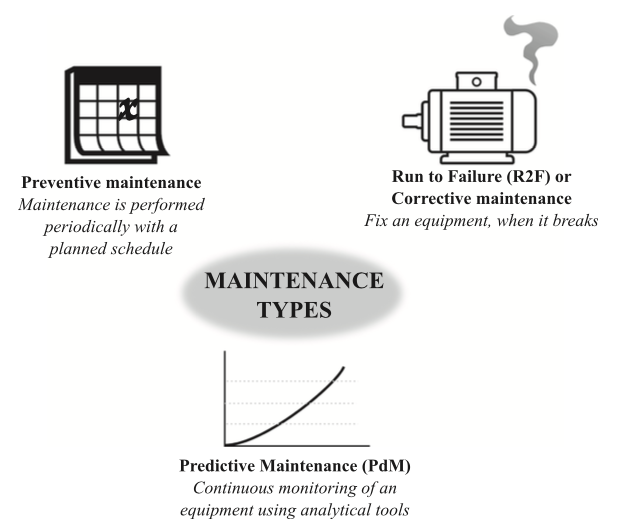
\includegraphics[scale=0.9]{TESI DI FIORE/img/maintenance_strategy_overview.png}
\centering
\caption{Overview of different maintenance strategies \cite{3SystematicLiteratureReviewML}}
\label{maintenance_strategy_overview}
\end{figure}

Therefore, an optimal maintenance strategy should improve the equipment conditions for a better quality of final products, reduces equipment failure rates to minimize downtime in production, maximizes equipment lifetime and minimizes the total costs. According to this, the PdM is the most promising strategy and the one that is under the researcher's spotlight in the last few years. \\ 
Citing the study realized by Thyago P. Carvalho et al. \cite{3SystematicLiteratureReviewML} and Weiting Zhang et al. \cite{2DataDrivenMaintenance}, the PdM methods are mainly divided into three categories: 
\begin{itemize}
\item{\textit{Model-Based Predictive Maintenance} consists in the development of complex mathematical models which replicate the behaviour of an equipment and its degradation process.}
\item{\textit{Knowledge-Based Predictive Maintenance} consists in the application of threshold-based rules, built on some measurements taken from machines, and that generate alerts in case in which some of them cross the thresholds.}
\item{\textit{Data-Based or Data-Driven Predictive Maintenance} makes the use of progresses reached in the fields of advanced analytic and artificial intelligence (AI) techniques to build machine learning (ML) or deep learning (DL) models that have the capability to predict when next failures will occur. }
\end{itemize}

It is good to clarify that behind the word "predictive" several meanings are hidden. In data-driven techniques the main goal is to train ML or DL models on historical data, which contains information about the degradation of a component or about normal or anomalous behaviour of an equipment, and then use them to predict its remaining useful life (RUL) or to detect some anomalies and generate alerts. Obviously this category of PdM is boosted by the paradigm of Industry 4.0 thanks to the large amount of historical or real-time time-series data collected by sensors in smart factories, allowing ever better performances.\\
The main drawback of using Industry 4.0 paradigm, especially to enable predictive maintenance, is the cost of digitalization, but fortunately in last years European Governments has started to support this transition defining new and accurate plans of investment in research and development. For example, the Italian government, with the "New Transition Plan 4.0", published in 2020 and valid for the next three years, is going to invest around 24 billion euros to promote the digital transition and to support investments by private companies \cite{12MiseNuovoPianoTransizione}.\\ 
In conclusion, regarding tangible results of the transition, is worth analyzing the Figure \ref{predictive_maintenance_reduction_costs}, taken from the study made by Porsche Consulting \cite{11PorscheStudy}, which results show a significant reduction in maintenance costs through implementation of predictive systems.

\begin{figure}[ht]
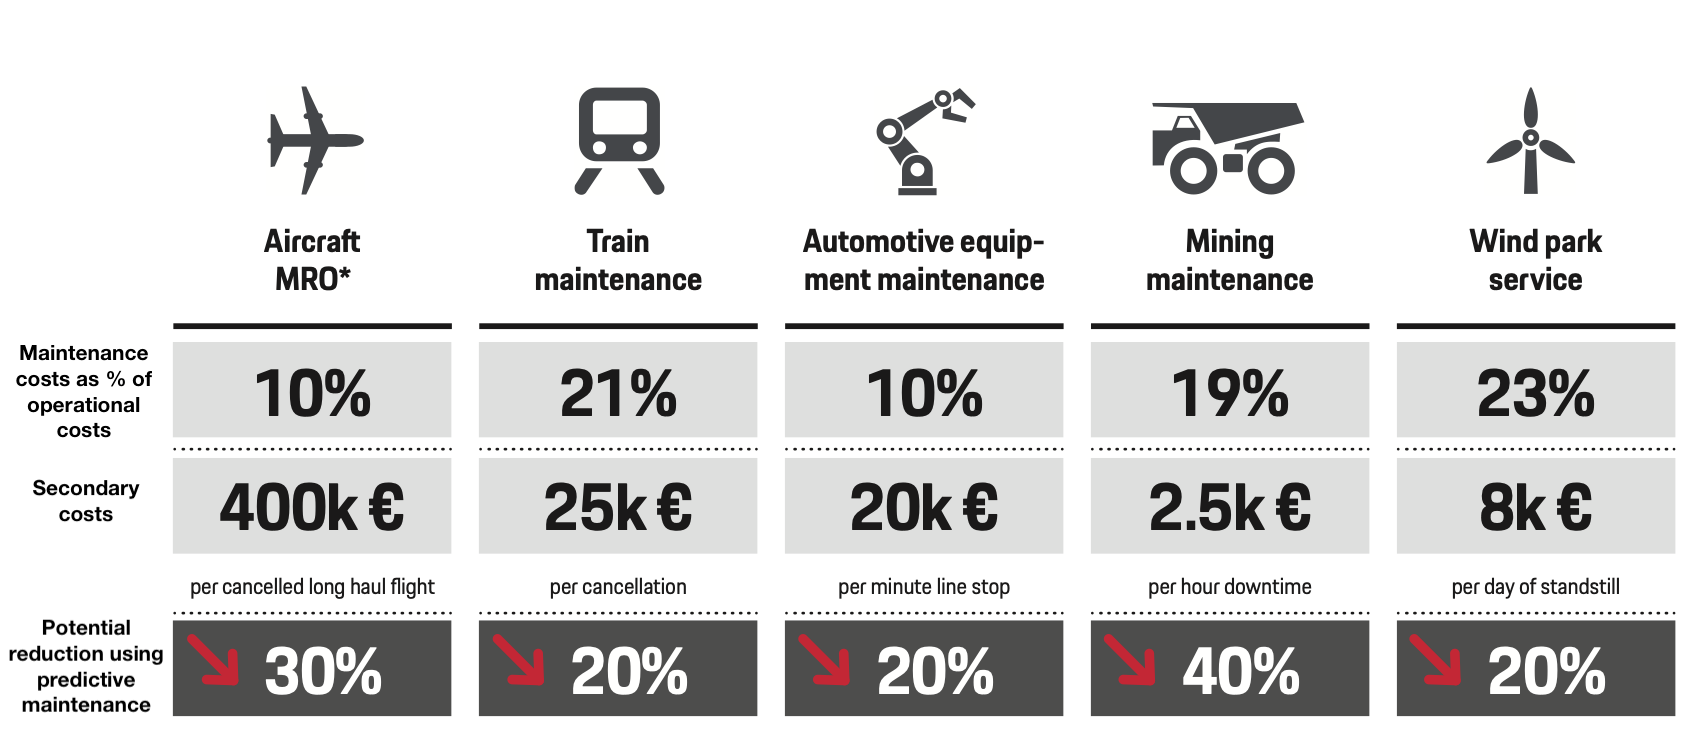
\includegraphics[scale=0.4]{TESI DI FIORE/img/UsingPredictiveMaintenanceCostReduction.png}
\centering
\caption{Potential overview for maintenance cost reduction across five industries \cite{11PorscheStudy}}
\label{predictive_maintenance_reduction_costs}
\end{figure}


\section{Anomaly Detection in PdM}
Anomaly detection (or outlier detection) is a set of techniques for the identification of anomaly patterns in data that deviates from normal behaviour. For example, a machine, like a pump or a steam turbine, after a period of normal behaviour starts deteriorating due to regular use, generating some \textit{anomalies} and entering in a status that can be identified as anomalous. This state should not be considered as a total failure state (in such case the machine should be turned off) but as a warning state, indicating that some maintenance procedures are needed \cite{5AnomalyDetectionSurvey}. Anomaly detection is so used to minimize the cost of failures, discovering anomalous behavior of mechanical devices in the production line in order to predict potential problems as early as possible. In this way, the production plans can be adjusted accordingly to avoid failures, and the failures already happened can be contained in their early stage to avoid cascading effects.\\
As for the PdM in general, in last years, in the context of anomaly detection, different ML and DL techniques have been developed. Most of them are based on time-series, which represents historical or real-time measurements of different parameters recorded in sequence from machines by smart sensors. In this type of data, three different kinds of anomaly can be identified \cite{6AnomalyIoTTimeSeries}: 
\begin{itemize}
\item{\textit{Point anomaly}: the time-series returns in normal state in very short time period, so the anomaly is represented by only few observations;}
\item{\textit{Contextual anomalies}: observation or sequences that deviates from expected patterns, but if taken in isolation they not exceed the range of expected values for that signal;}
\item{\textit{Collective or Pattern Anomalies}: observations that are labeled as anomalous only if taken together.}
\end{itemize}
In the Figure \ref{anomalies} can be found a graphical view of the just mentioned anomaly types. 
\begin{figure}[ht]
\centering
\begin{subfigure}
    \centering
    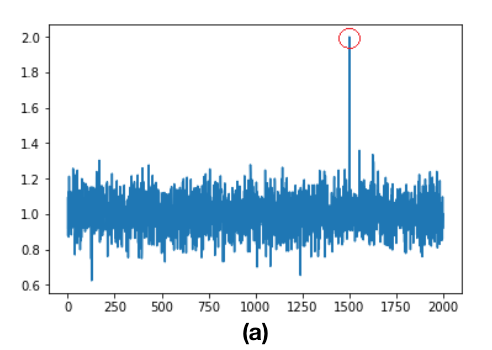
\includegraphics[scale=0.51]{TESI DI FIORE/img/anomaly_a.png}
\end{subfigure}
\begin{subfigure}
    \centering
    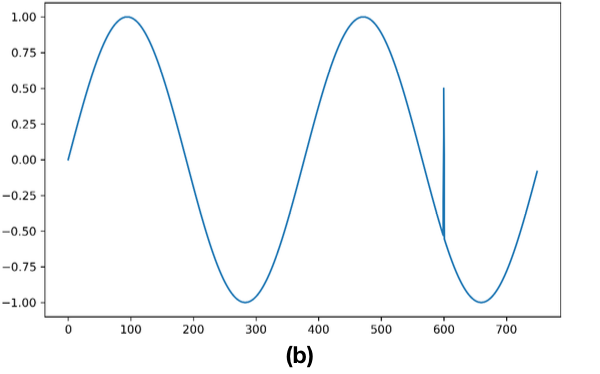
\includegraphics[scale=0.45]{TESI DI FIORE/img/anomaly_b.png}
\end{subfigure}
\begin{subfigure}
    \centering
    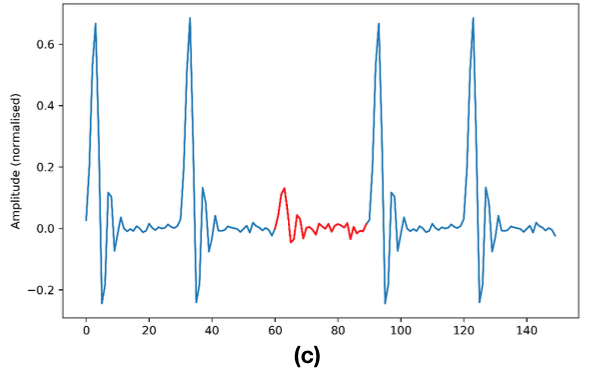
\includegraphics[scale=0.45]{TESI DI FIORE/img/anomaly_c.png}
\end{subfigure}
\caption{Point anomaly (a), contextual anomaly (b) and collective anomaly (c) \cite{6AnomalyIoTTimeSeries}.}
\label{anomalies}
\end{figure}

\section{Challenges of Anomaly Detection}
Being a field of predictive maintenance, also in anomaly detection there are some important elements that must be taken into consideration, because they influence the performances of trained models.
\subsection{Contextual information}
The presence of a variety of sensors, distributed around the environment of the monitored system, gives the opportunity to include contextual information into the collected data, allowing the improvement of the anomaly detection process performances. In particular, two types of contexts must be handled: spatial context and external context. When multiple sensors are deployed to monitor a system that moves in different environment conditions, such as a train, the contextual information can effect a lot the performances of an anomaly detector. For example some behaviours that are normal when a train is running on a flat ground can be anomalous when it is climbing an incline. This problem could be resolved using an accelerometer that measures the angle with the ground and incorporate its observations during the training. Moreover, external context can be likewise effective when monitoring the internal temperature of an equipment, because in this case the knowledge of external temperature can effect the results of the detection in better. Obviously, taking in consideration the context, some drawbacks are present, for example the necessity to build a more complex and expensive monitoring system and a more difficulty in model training.
\subsection{Data dimensionality and noise}
Other important elements that must be taken in consideration into the development of an anomaly detector are the data dimensionality and measurements noise. Regarding data dimensionality, there are two different cases: univariate or multivariate data. Univariate data consists of observations recorded by a single sensor, while multivariate data consists of a sequence of observations recorded by multiple sensors. In the first case, machine learning models must be trained to discover the historical relationships that could be hidden in the sequence of values recorded by one sensor. In the second case, observations recorded by more than one sensor are linked together by the timestamp. This can be regarded as an advantage in some situations in which patterns are hidden between the relationships among the various physical measures monitored by sensors. Regarding the noise, in an IoT environment where a large number of low cost, resource constrained sensors are deployed, the data quality is often affected by significant disturbs, inconsistencies and missing or duplicated data. Where the sensors are powered by battery, these challenges are often amplified as the available charge decreases. These problems can be resolved aggregating data from multiple similar sensors into a single observation to reduce the environmental noise.
\subsection{Stationarity}
Stationarity is also another important element that needs to be treated: a stationary time-series is one where the mean, variance and autocorrelation does not vary with time. Unfortunately, in real world non-stationary time series are very frequent and this make more complex the training of AI models because statistical data stream distribution may vary over time and so what is normal over a period of time could be anomalous in another (concept of seasonality).
\subsection{Lack of anomalous data}
One last challenge, maybe the most important that must be faced in anomaly detection, is the prediction of the "unknown". The word "unknown" refers to undesirable (or anomalous) events of which available data are not enough. The consequence is that ML and DL models can not be trained using a classification approach, because only normal state monitored data of an equipment are available to build an anomaly detector \cite{7AnomalyDetectionUnsupervised}. In fact, for example, while it is possible to build a toy industrial machine in order to collect data of its normal and anomalous working states, on the other hand, in some situations, it is unthinkable, dangerous and expensive try to generate anomalous behaviors of a machinery used in real world, like an aircraft engine, a train engine or an industrial press, with the only goal of collecting data. Moreover, even if anomalous data are available, they not surely represent all the anomalous situations in which the machine under investigation could be, because the space of the anomalies is very irregular and it is practically impossible to have a complete vision of them in order to trains models with a classification approach.

\section{Unsupervised Anomaly Detection}
Because is quite simple to collect large dataset associated to a particular machine's working state, in such situations, ML and DL models must be trained in a unsupervised way, where the word unsupervised means that the models try to detect an events that have no examples in the data history used for training \cite{8AnomalyDetectionUnsupervised2}. At this point, a question that arises is: how a trained model could detect never seen anomalous measurements and generate alerts? A possible approach is showed in Figure \ref{scoring_system_approach}. The figure shows that models could be trained to reconstruct the received input, that refers to a normal working state, and if the output is enough different from the input an alert will be triggered.

\begin{figure}[ht]
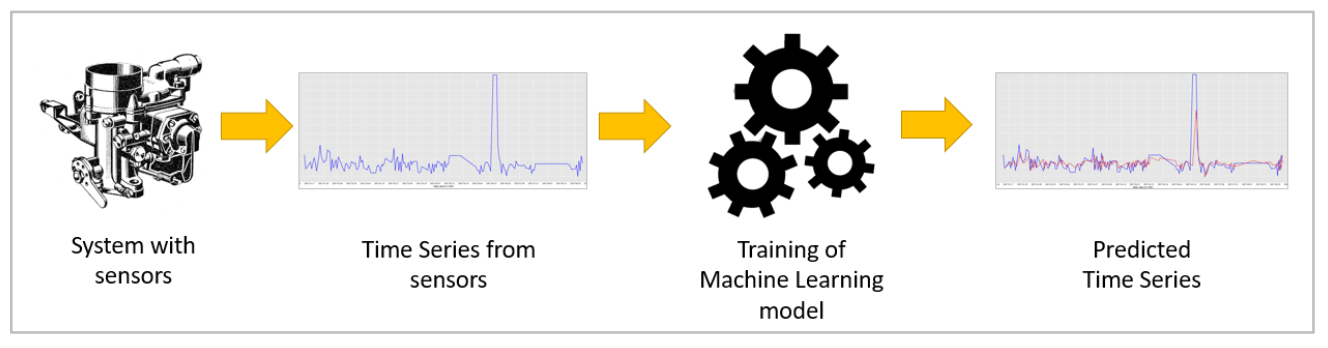
\includegraphics[scale=0.65]{TESI DI FIORE/img/UnsupervisedLearningAnomalyDetection.png}
\centering
\caption{Anomaly detection high level workflow \cite{7AnomalyDetectionUnsupervised}}
\label{scoring_system_approach}
\end{figure}

Anomalies in sensor data can be defined as previously unseen patterns and the algorithm for anomaly detection should be able to detect known anomalies as well as generalize to new and unknown ones. In general, a common approach to achieve this detection is a sliding-window (Figure \ref{anomaly_detection_with_sliding_window}). Since models are trained on normal data which is a fixed-length sequence of preceding steps, it can achieve anomaly detection by comparing the predicted value at each timestep with the actual sequence, allowing also to perform a real-time detection and eventually alerts generation \cite{9UnsupervisedOnlineAnomalyDetectionMultivariate} and, moreover, using the temporal relationships present in sequences.
\begin{figure}[ht]
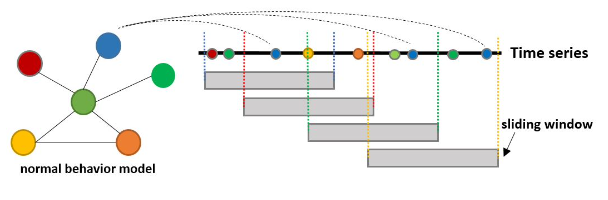
\includegraphics[scale=0.8]{TESI DI FIORE/img/OnlineAnomalyDetection.png}
\centering
\caption{Online detection procedure with sliding window \cite{9UnsupervisedOnlineAnomalyDetectionMultivariate}}
\label{anomaly_detection_with_sliding_window}
\end{figure}
Several approaches have been developed for unsupervised anomaly detection. R. Silipo et al \cite{8AnomalyDetectionUnsupervised2} describes two techniques: the first, named Control Chart, and the second based on Auto-Regressive (AR) models. In the first case, the boundaries for an anomaly-free functioning equipment are defined. This boundaries are usually centered on the average signal values recorded by sensors and bounded by twice the standard deviation in both directions. If the signal is wandering off this anomaly free area, an alarm should occur. The second approach is conceptually similar to the Control Chart and uses this anomaly-free time window to train an AR model. The boundaries for anomaly-free functioning are defined here on the prediction errors on the training set. To clarify, the model receives in input a time-series made by sensor observations and the next time-step value is then predicted by the model. Successively, according a threshold established using the training set, if the predicted value is enough different from the actual value, an alarm is fired off requiring further checkups. This second technique is also cited in the survey \cite{6AnomalyIoTTimeSeries}.\\
Another important and suitable machine learning method for this task is \textbf{autoencoder} and for this reason it will be at the center of this discussion. 
An autoencoder (Figure \ref{autoencoder_image}) is a neural network mainly designed to encode the input into a compressed and meaningful representation and then decode it back, such that the reconstructed input is as much as similar to the original one \cite{10Autoencoders}.\\
\begin{figure}[ht]
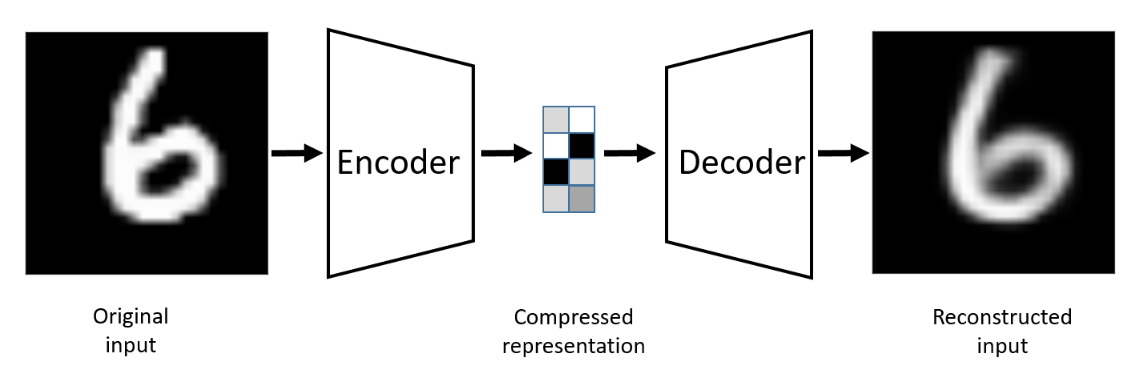
\includegraphics[scale=0.65]{TESI DI FIORE/img/Autoencoder.png}
\centering
\caption{An autoencoder example \cite{10Autoencoders}.}
\label{autoencoder_image}
\end{figure}
Autoencoder is so an unsupervised technique because any label or class is needed for training phase, so it results a perfect approach for anomaly detection. In details, the encoder part is made of a series of layers with a decreasing number of nodes and ultimately reduces data into a latent vector, which represents a reduced (encoded) version of the input and which contains only valuable or essential information of it. The decoder, as the encoder, is made of different layers with an increasing number of nodes. It is trained to receive in input the latent vector and to generate an output as much as possible similar to the input. The process is described in mathematical way as follow:
\[argmin_{D,E} || X - D(E(X))||\]
Where X is the input data, E is an encoder network, and D is a decoder network. Using this formula is evident that the performances of an autoencoder are evaluated using the reconstruction error: the difference between the input and the output in terms of mean absolute error (MAE) or mean squared error (MSE).\\
Summarizing, in the context of anomaly detection in predictive maintenance, the autoencoder can be trained to reconstruct the normal observations collected from a working machine in normal working state. Next, in detection phase, its reconstruction error can be used as an anomaly score: if it is under a threshold the observation in input can be classified as normal, otherwise as anomalous. As mentioned before for AR models, the threshold is found using the reconstruction error of training set samples or using different techniques.\\
The next chapter presents different autoencoder approaches in anomaly detection, with a particular focus on anomalous sound detection tasks.

